%
\chapter{Zemeljski sistemi za določanje lastnega položaja}
\label{Ch:LastPolZem} % Always give a unique label
% use \chaptermark{}
% to alter or adjust the chapter heading in the running head

Radijsko navigacijo izvajamo s pomočjo ocenjevanja razdalj do oddajnikov. Oddajniki so razporejeni na ključnih položajih na zemeljskem površju, njihove koordinate v ravnini Zemlje so znane. Če je sprejemnik sposoben izmeriti čas potovanja signala od vsaj dveh oddajnikov do sebe in časa potovanj preračunati v oceni razdalj, že lahko oceni svoj položaj v ravnini koordinatnega sistema. 

Tehnologija prvih radijskih navigacijskih zemeljskih sistemov se je osredotočala na medsebojno sinhronost ur oddajnikov in stabilnost takta merilnika časa v sprejemniku ni pa zahtevala sinhronosti merilnikov časa v sprejemniku z urami v oddajnikih (primerjaj z rešitvijo v poglavju GNSS). 

Torej zaradi težav s stalnim preverjanjem usklajenosti ur oddajnikov in sprejemnikov se v praksi merijo razlike v časih signalov prispetij v sprejemnik in ne časi potovanj od oddajnikov do sprejemnikov. Ker sprejemnik ve (ima zabeležene koordinate) odkod so bili signali oddani, lahko iz časovnih razlik nariše hiperboloide - v njihovem presečišču je navigacijska rešitev oz. sprejemnik. Negotovost določanja položaja so povzročale neusklajenosti ur in spreminjanje pogojev razširjanja signalov. Zaradi precejšnje negotovosti takih sistemov v preteklosti (Loran-C), so po nastopu GNSS zemeljski sistemi zamrli. Potrebe po rezervnem sistemu, ki bi v primeru težav nadomestil GNSS, so v uporabi ohranile potomca sistema Loran-C, ki se imenuje e-Loran. Poleg kanala za prenos časovno-prožilnih signalov uporablja e-Loran tudi kanal za prenos podatkov o pogojih za razširjanje siganlov.    

%Prednost sledenja več signalom je, da sprejemnik zna oceniti ali naj uporabnik zaupa navigacijski rešitvi ali ne. Sprejemnik sistema e-Loran je sposoben sprejeti in dekodirati sporočilo tudi po podatkovnem kanalu in uporabiti popravke, ki jih dobi po tej poti. Pulzi e-Lorana temeljijo na pulzih Loran-C. Sistem e-Loran zajema modernizirana kontrolna središča z bolj stabilnimi izvori časa, svetilnike in nadzorne postaje. lastna oznaka postaje, čas oddaje, opozorila o trenutnih nepravilnostih razširjanja pulzov, sporočila o istovetnosti oddanih pulzov in popravki za izboljšanje sprejemanja. Prav zaradi dodatnih informacij v podatkovnem kanalu se smejo navigacijske naprave e-Loran uporabljati za določanje položaja pri vplutju v pristanišča. Točnost sistema e-Loran je od 0,004 do 0,01 NM, to je od 8 do 20 m. Prehod na e-Loran omogoča uporabo sprejemnikov Loran-C, vendar z njimi ni možno izkoristiti prednosti e-Lorana, saj sprejemniki Loran-C ne poznajo podatkovnega kanala. Potreben je pač poseben sprejemnik.

%V času pisanja te diplomske naloge je prihodnost e-Lorana kot rezervnega navigacijskega sistema in vira točnega časa še neznana. Ugasnili so svetilnike v zahodni Evropi in v ZDA, od evropskih delujejo le še svetilniki v Veliki Britaniji, uporabljajo pa jih še v Aziji. Čeprav je vzdrževanje e-Lorana relativno poceni, države še tehtajo možnosti za nadaljnji obstoj. (USCG, 2007)

\begin{figure*}[!ht]
	\begin{center}
		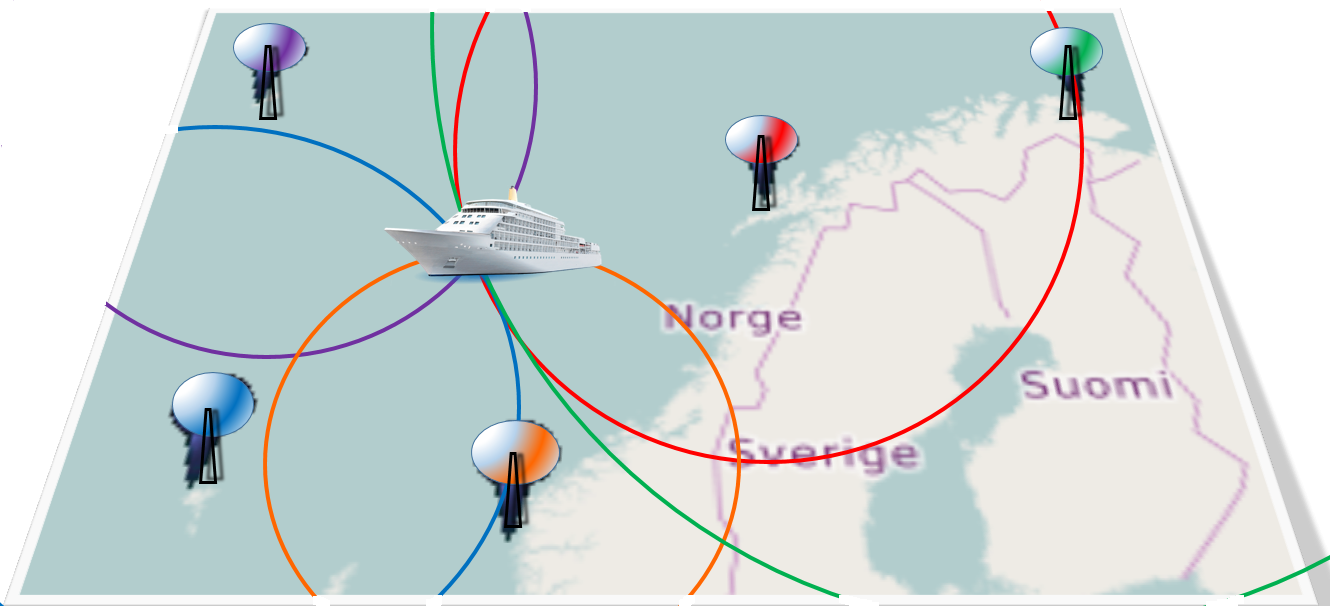
\includegraphics[height=4cm]{Predavanja/04_ZemeljLastPolozaj/figs/LoranstationsEuropeDetDetSign_20160925.png}  
		\caption{Prikaz multilateracije delujočih postaj Loran-C}\label{Fig_MultiLoranC}
	\end{center}
\end{figure*}


%https://en.wikipedia.org/wiki/Loran-C
%Stations Listed https://tools.wmflabs.org/osm4wiki/cgi-bin/wiki/wiki-osm.pl?project=en&article=Loran-C
% LORAN-C transmitters operate at peak powers of 100–4,000 kilowatts, comparable to longwave broadcasting stations. Most use 190–220 metre tall mast radiators, insulated from ground. The masts are inductively lengthened and fed by a loading coil (see: electrical lengthening). A well known-example of a station using such an antenna is Rantum. Free-standing tower radiators in this height range are also used[clarification needed]. Carolina Beach uses a free-standing antenna tower. Some LORAN-C transmitters with output powers of 1,000 kW and higher used supertall 412 metre mast radiators (see below). Other high power LORAN-C stations, like George, used four T-antennas mounted on four guyed masts arranged in a square.

%All LORAN-C antennas are designed to radiate an omnidirectional pattern. Unlike longwave broadcasting stations, LORAN-C stations cannot use backup antennas because the exact position of the antenna is a part of the navigation calculation. The slightly different physical location of a backup antenna would produce Lines of Position different from those of the primary antenna.


%eLORAN[edit]
%With the perceived vulnerability of GNSS systems,[47] and their own propagation and reception limitations, renewed interest in LORAN applications and development has appeared.[48] Enhanced LORAN, also known as eLORAN or E-LORAN, comprises an advancement in receiver design and transmission characteristics which increase the accuracy and usefulness of traditional LORAN. With reported accuracy as good as ± 8 meters,[49] the system becomes competitive with unenhanced GPS. eLORAN also includes additional pulses which can transmit auxiliary data such as DGPS corrections. eLORAN receivers now use "all in view" reception, incorporating signals from all stations in range, not solely those from a single GRI, incorporating time signals and other data from up to 40 stations. These enhancements in LORAN make it adequate as a substitute for scenarios where GPS is unavailable or degraded.[50]

\section{Section Heading}
\label{sec:1}
% Always give a unique label
% and use \ref{<label>} for cross-references
% and \cite{<label>} for bibliographic references
% use \sectionmark{}
% to alter or adjust the section heading in the running head
Your text goes here. Use the \LaTeX\ automatism for your citations
\cite{monograph}.

\subsection{Subsection Heading}
\label{sec:2}
Your text goes here.

\begin{equation}
\vec{a}\times\vec{b}=\vec{c}
\end{equation}

\subsubsection{Subsubsection Heading}
Your text goes here. Use the \LaTeX\ automatism for cross-references as
well as for your citations, see Sect.~\ref{sec:1}.

\paragraph{Paragraph Heading} %
Your text goes here.

\subparagraph{Subparagraph Heading.} Your text goes here.%
%
\index{paragraph}
% Use the \index{} command to code your index words
%
% For tables use
%
\begin{table}
\centering
\caption{Please write your table caption here}
\label{tab:1}       % Give a unique label
%
% For LaTeX tables use
%
\begin{tabular}{lll}
\hline\noalign{\smallskip}
first & second & third  \\
\noalign{\smallskip}\hline\noalign{\smallskip}
number & number & number \\
number & number & number \\
\noalign{\smallskip}\hline
\end{tabular}
\end{table}
%
%
% For figures use
%
\begin{figure}
\centering
% Use the relevant command for your figure-insertion program
% to insert the figure file.
% For example, with the option graphics use

\includegraphics[height=4cm]{figure}
%
% If not, use
%\picplace{5cm}{2cm} % Give the correct figure height and width in cm
%
\caption{Please write your figure caption here}
\label{fig:1}       % Give a unique label
\end{figure}
%
% For built-in environments use
%
\begin{theorem}
Theorem text goes here.
\end{theorem}
%
% or
%
\begin{lemma}
Lemma text goes here.
\end{lemma}
%
%
% Problems or Exercises should be sorted chapterwise
\section*{Problems}
\addcontentsline{toc}{section}{Problems}
%
% Use the following environment.
% Don't forget to label each problem;
% the label is needed for the solutions' environment
\begin{prob}
\label{prob1}
The problem\footnote{Footnote} is described here. The
problem is described here. The problem is described here.
\end{prob}

\begin{prob}
\label{prob2}
\textbf{Problem Heading}\\
(a) The first part of the problem is described here.\\
(b) The second part of the problem is described here.
\end{prob}



%
